\documentclass[8pt,a4paper]{article}
\usepackage[a4paper, margin=1in]{geometry}
\usepackage[utf8]{inputenc}
\usepackage{amsmath}
\usepackage{amsfonts}
\usepackage{amssymb}
\usepackage{graphicx}
\usepackage{float}
\usepackage{pdfpages}
\usepackage[makeroom]{cancel}
\begin{document}
	
	\title{Symplectic Algorithms}
	\author{James Bounds}
	\maketitle
	
	For this project we will consider a central force of type
	\begin{equation}
		\nabla V(\mathbf{r}) = -f(r) \mathbf{\hat{r}}
	\end{equation}
	which is formed from a potential solely dependent on the distance from the coordinate origin
	\begin{equation}
		r=|\mathbf{r}|
	\end{equation}
	
	\section{Angular Momentum Conservation}
	The action of any sequential updating algorithm can be formed by an appropriate combination of two fundamental algorithms. Therefore by showing that each of the fundamental algorithms conserve angular momentum, we can show that any sequential updating algorithm respects the conservation of angular momentum.
	\subsection{Cromer Algorithm}
	The Cromer method for a given time-step $\Delta t$ is given by
	\begin{align} \label{cromer}
		\mathbf{v}_{n+1} &= \mathbf{v}_n + \mathbf{a} (\mathbf{r_n}) \,\Delta t \nonumber \\
		\mathbf{r}_{n+1} &= \mathbf{v}_n + \mathbf{v}_{n+1} \,\Delta t
	\end{align}
	The angular momentum at the $(n+1)^\mathrm{th}$ step is given by
	\begin{align}
		\mathbf{L}_{n+1} &= \mathbf{r}_{n+1} \times \mathbf{v}_{n+1} \nonumber \\
		&= \Big(\mathbf{r}_n + \mathbf{v}_n \Delta t\Big) \times
		\Big(\mathbf{v}_n + \mathbf{a}(\mathbf{r}_n) \Delta t\Big) \nonumber \\
		&= \mathbf{r}_n\times\mathbf{v}_n + \mathbf{v}_{n+1}\times\mathbf{v}_n \Delta t + \underbrace{\cancel{\mathbf{r}_n \times \mathbf{a}(\mathbf{r}_n)}}_{\text{Central Force}}\Delta t + \mathbf{v}_{n+1} \times \mathbf{a}(r_n) \Delta t ^2 \nonumber \\
		&= \mathbf{r}_n\times\mathbf{v}_n + \mathbf{v}_{n+1}\times\mathbf{v}_n \Delta t + \mathbf{v}_{n+1} \times \mathbf{a}(r_n) \Delta t ^2 \nonumber \\
		&= \mathbf{r}_n\times\mathbf{v}_n + \mathbf{v}_{n+1}\times \Big(\mathbf{v}_n + \mathbf{a}(r_n) \Delta t \Big) \Delta t \nonumber \\
		&= \mathbf{r}_n\times\mathbf{v}_n + \underbrace{\cancel{\mathbf{v}_{n+1}\times \mathbf{v}_{n+1}}}_{\text{Vanishes Identically}} \Delta t \nonumber \\
		&= \mathbf{r}_n\times\mathbf{v}_n \nonumber \\
		\mathbf{L}_{n+1}	&= \mathbf{L}_n
	\end{align}
	Thus we observe that each step of the Cromer algorithm preserves angular momentum independently of the time-step size.
	
	This algorithm forms the conjugate to the other fundamental sequential algorithm, the Newton algorithm. We showed in our previous project that the Newton method is actually the same as the Cromer algorithm, but run in reverse. We could therefore argue that the angular momentum in the Newton algorithm is also preserved just as the above expressions show that we have conservation in the direction $\mathbf{L}_{n+1} \rightarrow \mathbf{L}_n$. We show explicitly that angular momentum is preserved by the Newton algorithm in the next section.
	\subsection{Newton Algorithm}
	The Newton algorithm for a given time-step $\Delta t$ is given by
	\begin{align} \label{newton}
		\mathbf{r}_{n+1} &= \mathbf{r}_n + \mathbf{v}_n \, \Delta t \nonumber \\
		\mathbf{v}_{n+1} &= \mathbf{v}_n + \mathbf{a}(\mathbf{r}_{n+1}) \, \Delta t \nonumber \\
	\end{align}
	Angular momentum at the $(n+1)^\mathrm{th}$ step is given by
	\begin{align}
		\mathbf{L}_{n+1} &= \mathbf{r}_{n+1} \times \mathbf{v}_{n+1} \nonumber \\
		&= \Big(\mathbf{r}_n + \mathbf{v}_n \Delta t\Big) \times \Big(\mathbf{v}_n + \mathbf{a}(\mathbf{r}_{n+1})\Delta t\Big) \nonumber \\
		&= \mathbf{r}_n \times \mathbf{v}_n + \mathbf{r}_n \times \mathbf{a}(\mathbf{r}_{n+1})\Delta t + \underbrace{\cancel{\mathbf{v}_n\times\mathbf{v}_n}\Delta t}_{\text{Vanishes Identically}} + \mathbf{v_n}\times\mathbf{a}(\mathbf{r}_{n+1}) \Delta t ^2 \nonumber \\
		&= \mathbf{r}_n \times \mathbf{v}_n + \mathbf{r}_n \times \mathbf{a}(\mathbf{r}_{n+1})\Delta t + \mathbf{v_n}\times\mathbf{a}(\mathbf{r}_{n+1}) \Delta t ^2 \nonumber \\
		&= \mathbf{r}_n \times \mathbf{v}_n + \Big(\mathbf{r}_n + \mathbf{v_n}\Delta t\Big)\times\mathbf{a}(\mathbf{r}_{n+1}) \Delta t \nonumber \\
		&= \mathbf{r}_n \times \mathbf{v}_n + \underbrace{\cancel{\mathbf{r}_{n+1}\times\mathbf{a}(\mathbf{r}_{n+1})}}_{\text{Central Force}} \Delta t \nonumber \\
		&= \mathbf{r}_n \times \mathbf{v}_n \nonumber \\
		\mathbf{L}_{n+1}	 &= \mathbf{L}_n					 
	\end{align}
	We that that in the case of a central force, the newton algorithm conserves angular momentum at every iteration, regardless of the size of time-step. The order in which we observe the cancellations was exactly reversed from the Cromer algorithm, reflecting that the two are time reverses of one another.
	
	\section{Operator Definitions}
	We define the translation operator $\hat{T}$ and the "velocitation" operator $\hat{V}$ as the following displacements
	\begin{align}
		\hat{T} &= \mathbf{v}\cdot \frac{\partial}{\partial \mathbf{r}} \\
		\hat{V} &= \mathbf{a}(\mathbf{r})\cdot \frac{\partial}{\partial \mathbf{v}}
	\end{align}
	
	\subsubsection{Cromer Operator $T_\mathrm{1a}$}
	We can show that the Cromer method is equivalent to the action of the operator
	\begin{equation}
		\hat{T}_\mathrm{1a} = e^{\epsilon \hat{V}} e^{\epsilon \hat{T}}
	\end{equation}
	We demonstrate the action of this operator on a trajectory point
	\begin{align}
		\hat{T}_\mathrm{1a}
		\begin{pmatrix}
			\mathbf{r} \\ \mathbf{v}
		\end{pmatrix}
		&= e^{\epsilon \hat{V}} e^{\epsilon \hat{T}}
		\begin{pmatrix}
			\mathbf{r} \\ \mathbf{v}
		\end{pmatrix} \nonumber \\
		&= e^{\epsilon \hat{V}}
		\begin{pmatrix}
			\mathbf{r} + \epsilon \mathbf{v} \\ \mathbf{v}
		\end{pmatrix} \nonumber \\
		&=
		\begin{pmatrix}
			\mathbf{r} + \epsilon (\mathbf{v} + \epsilon\mathbf{a}(\mathbf{r}))\\
			\mathbf{v} + \epsilon\mathbf{a}(\mathbf{r})
		\end{pmatrix}
	\end{align}
	
	\subsubsection{Newton Operator $\hat{T}_\mathrm{1b}$}
	We can show that the Newton method is equivalent to the action of the operator
	\begin{equation}
		\hat{T}_\mathrm{1b} = e^{\epsilon \hat{T}} e^{\epsilon \hat{V}}
	\end{equation}
	We demonstrate the action of this operator on a trajectory point
	\begin{align}
		\hat{T}_\mathrm{1a}
		\begin{pmatrix}
			\mathbf{r} \\ \mathbf{v}
		\end{pmatrix}
		&= e^{\epsilon \hat{T}} e^{\epsilon \hat{V}}
		\begin{pmatrix}
			\mathbf{r} \\ \mathbf{v}
		\end{pmatrix} \nonumber \\
		&= e^{\epsilon \hat{T}}
		\begin{pmatrix}
			\mathbf{r} \\
			\mathbf{v} + \epsilon\mathbf{a}(\mathbf{r})
		\end{pmatrix} \nonumber \\
		&=
		\begin{pmatrix}
			\mathbf{r} + \epsilon \mathbf{v} \\
			\mathbf{v + \epsilon\mathbf{a}(\mathbf{r} + \epsilon \mathbf{v})}
		\end{pmatrix} \nonumber \\
	\end{align}
	
	With these operator definitions, it is now trivial to see that the Newton and Cromer methods are time inverses of one another
	\begin{equation}
		\hat{T}_\mathrm{1a}(\epsilon) \hat{T}_\mathrm{1b}(-\epsilon) = \hat{T}_\mathrm{1b}(\epsilon) \hat{T}_\mathrm{1a}(-\epsilon)  = 1
	\end{equation}
	
	\subsubsection{Position Verlet operator $\hat{T}_\mathrm{PV}$}
	The second order symplectic methods can be formed by making time-reversal symmetric combinations of the fundamental operators $\hat{T}_\mathrm{1a}$ and $\hat{T}_\mathrm{1b}$. We will see that the position Verlet method is equivalent to the action of the operator
	
	\begin{equation}
		\hat{T}_\mathrm{PV} = \hat{T}_\mathrm{1b}\left(\frac{\epsilon}{2}\right) \hat{T}_\mathrm{1a}\left(\frac{\epsilon}{2}\right) = e^{\epsilon \hat{T}/2}e^{\epsilon \hat{V}} e^{\epsilon \hat{T}/2}
	\end{equation}
	The action of this operator on a trajectory point is
	\begin{align}
		\hat{T}_\mathrm{PV}
		\begin{pmatrix}
			\mathbf{r} \\ \mathbf{v}
		\end{pmatrix}
		&= e^{\epsilon \hat{T}/2}e^{\epsilon \hat{V}} e^{\epsilon \hat{T}/2}
		\begin{pmatrix}
			\mathbf{r} \\ \mathbf{v}
		\end{pmatrix} \nonumber \\
		&= e^{\epsilon \hat{T}/2}e^{\epsilon \hat{V}}
		\begin{pmatrix}
			\mathbf{r} + \epsilon \mathbf{v}/2  \\
			\mathbf{v}
		\end{pmatrix} \nonumber \\
		&= e^{\epsilon \hat{T}/2}
		\begin{pmatrix}
			\mathbf{r} + \epsilon (\mathbf{v} + \epsilon\mathbf{a}(\mathbf{r}))/2  \\
			\mathbf{v} + \epsilon\mathbf{a}(\mathbf{r})
		\end{pmatrix} \nonumber \\
		&=
		\begin{pmatrix}
			(\mathbf{r} + \epsilon \mathbf{v}/2) + \epsilon [\mathbf{v} + \epsilon\mathbf{a}(\mathbf{r} + \epsilon \mathbf{v}/2)]/2  \\
			\mathbf{v} + \epsilon\mathbf{a}(\mathbf{r} + \epsilon \mathbf{v}/2)
		\end{pmatrix}
	\end{align}
	We can see that this is the position Verlet method
	\begin{align}
		\mathbf{r}'  &= \mathbf{r}_n + \mathbf{v}_{n} \epsilon /2\nonumber \\
		\mathbf{v}_{n+1} &= \mathbf{v}_n + \mathbf{a}(\mathbf{r}') \, \epsilon \nonumber \\
		\mathbf{r}_{n+1} &= \mathbf{r}' + \mathbf{v}_{n+1} \epsilon/2
	\end{align}
	
	\subsubsection{Velocity Verlet operator $\hat{T}_\mathrm{VV}$}
	We will see that the velocity Verlet method is equivalent to the action of the time-reversal symmetric operator
	
	\begin{equation}
		\hat{T}_\mathrm{VV} = \hat{T}_\mathrm{1a}\left(\frac{\epsilon}{2}\right) \hat{T}_\mathrm{1b}\left(\frac{\epsilon}{2}\right) = e^{\epsilon \hat{V}/2}e^{\epsilon \hat{T}} e^{\epsilon \hat{V}/2}
	\end{equation}
	The action of this operator on a trajectory point is
	\begin{align}
		\hat{T}_\mathrm{VV}
		\begin{pmatrix}
			\mathbf{r} \\ \mathbf{v}
		\end{pmatrix}
		&= e^{\epsilon \hat{V}/2}e^{\epsilon \hat{T}} e^{\epsilon \hat{V}/2}
		\begin{pmatrix}
			\mathbf{r} \\ \mathbf{v}
		\end{pmatrix} \nonumber \\
		&= e^{\epsilon \hat{V}/2}e^{\epsilon \hat{T}}
		\begin{pmatrix}
			\mathbf{r} \\ 
			\mathbf{v} + \epsilon\mathbf{a}(\mathbf{r})/2
		\end{pmatrix} \nonumber \\
		&= e^{\epsilon \hat{V}/2}
		\begin{pmatrix}
			\mathbf{r} + \epsilon \mathbf{v} \\ 
			\mathbf{v} + \epsilon\mathbf{a}(\mathbf{r} + \epsilon \mathbf{v})/2
		\end{pmatrix} \nonumber \\
		&=
		\begin{pmatrix}
			\mathbf{r} + \epsilon (\mathbf{v} + \epsilon\mathbf{a}(\mathbf{r})/2) \\ 
			(\mathbf{v} + \epsilon\mathbf{a}(\mathbf{r})/2) + \epsilon\mathbf{a}(\mathbf{r} + \epsilon (\mathbf{v} + \epsilon\mathbf{a}(\mathbf{r})/2))/2
		\end{pmatrix} \nonumber \\
	\end{align}
	We see that this is equivalent to the velocity Verlet algorithm.
	\begin{align}
		\mathbf{v}' &= \mathbf{v} + \epsilon \mathbf{a}(\mathbf{r})/2 \\
		\mathbf{r}_{n+1} &= \mathbf{r}_n + \epsilon \mathbf{v}' \\
		\mathbf{v}_{n+1} &= \mathbf{v}'_n + \epsilon \mathbf{a}(\mathbf{r}_{n+1})/2
	\end{align}
	
	\section{Phase Space Volume}
	We consider the action of the translation operator $e^{\epsilon \hat{T}}$. We wish to see if the action of this operator is equivalent to a canonical transformation. The action of this operator is such that we have the transformation in 1-D
	\begin{equation}
		\begin{pmatrix}
			r_i \\
			p_i
		\end{pmatrix}
		\rightarrow
		\begin{pmatrix}
			r_i + p_i \epsilon \\
			p_i
		\end{pmatrix}
	\end{equation}
	We consider the newly affected coordinates as $R_i$, and $P_i$
	\begin{align}
		R_i &= r_i + p_i \epsilon \\
		P_i &= p_i
	\end{align}
	The Jacobian of this transformation is
	\begin{equation}
		\det
		\begin{pmatrix}
			\partial R_i/\partial r_i & \partial R_i/\partial p_i \\
			\partial P_i/\partial r_i & \partial P_i/\partial p_i
		\end{pmatrix}
		=\det
		\begin{pmatrix}
			1 & \epsilon \\
			0 & 1
		\end{pmatrix} = 1
	\end{equation}
	Since we are only updating a single coordinate, the determinant is always guaranteed to equal unity, implying that the translation operator action is always that of a canonical transformation.
	
	Similarly we can investigate the effect of the "velocitation" operator $e^{\epsilon\hat{V}}$. This operator is equivalent to the transformation
	\begin{align}
		R_i &= r_i \\
		P_i &= p_i + a(r_i) \epsilon
	\end{align}
	which is represented by the Jacobian
	\begin{equation}
		\det
		\begin{pmatrix}
			\partial R_i/\partial r_i & \partial R_i/\partial p_i \\
			\partial P_i/\partial r_i & \partial P_i/\partial p_i
		\end{pmatrix}
		=\det
		\begin{pmatrix}
			1 & 0 \\
			\epsilon\partial a/\partial r_i & 1
		\end{pmatrix} = 1
	\end{equation}
	Once again we see that this determinant is unity independently of time-step size, meaning this operator also represents a canonical transformation.
	
	We saw that any sequential updating step where only one coordinate is affected at a time always results in a canonical transformation. We also saw in previous section (and seen again in the Appendix) that any evolution operator which approximates the real evolution operator can be represented as a product of displacement operators each having a sequential update. Since the determinant of products is the product of determinants, the Jacobian for any transformation satisfying these requirements is unity and the transformation must be canonical.
	\section{Runge-Kutta-Nystrom Method}
	In this section, we plot the trajectory of two algorithms, one is the fourth order Runge-Kutta-Nystrom method (RKN4) and the other is the method we will refer to as $T_4$, defined by the operator
	\begin{equation} \label{T4}
		\hat{T}_4 = \frac{4}{3} \hat{T}_{\mathrm{VV}}^2(\Delta t /2) - \frac{1}{3}\hat{T}_\mathrm{VV}(\Delta t)
	\end{equation}
	For this comparison we use the initial conditions $\mathbf{r_0} = [x_0, 0]$ and $\mathbf{v_0} = [0, v_0]$, where $x_0=10$ and $v_0=0.1$.
	
	The geometric properties of the ellipse representing the exact solution can be derived from the given initial conditions and is expressed using the following relations.
	\begin{align*}
		p &= (x_0 v_0)^2 &= 1.0 \\
		e &= \sqrt{1-p/a} &= 0.9 \\
		E_0 &= \frac{1}{2}v_0^2 - \frac{1}{x_0} &= -0.095 \\
		a &= \frac{-1}{2E_0} &= 5.263 \\
		P &= 2\pi a^{3/2} &= 75.866
	\end{align*}
	
	We compare the result of using the two algorithms in Figure \ref{fig:p3-orbit} for the same initial conditions. It can be see that there is strong agreement between the resulting trajectories. In fact, on the scale of the whole orbit, the two solutions are essentially indistinguishable.
	\begin{figure}[H]
		\centering
		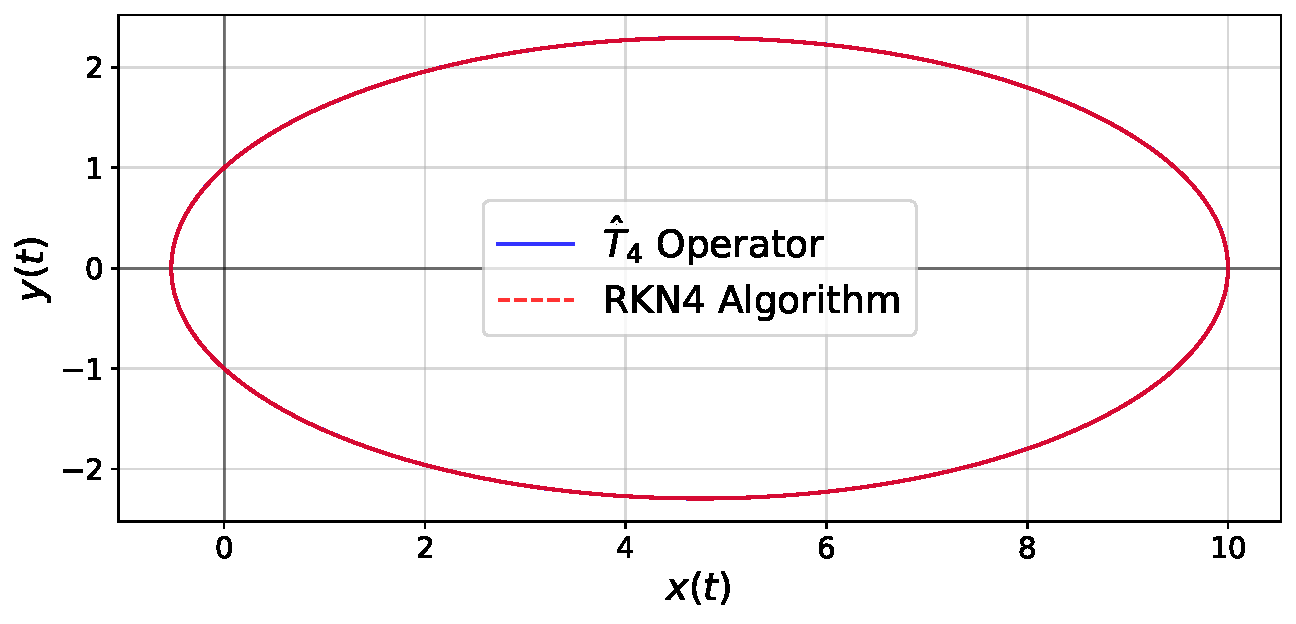
\includegraphics[width=1.0\linewidth]{diagrams/p3-orbit}
		\caption{Comparison of two trajectories. Both are started from the same initial conditions, but the trajectory shown in blue is propagated using the $\hat{T}_4$ operator in (\ref{T4}), and the trajectory shown in red is propagated using the 4th order Runge-Kutta-Nystrom (RKN4) algorithm. It can be seen that the two trajectories are essentially indistinguishable on this global scale. }
		\label{fig:p3-orbit}
	\end{figure}
	
	In order to elucidate imperceptible differences between the two solutions plotted in Figure \ref{fig:p3-orbit}, we subtract the two solutions at each time step. In the plots of Figure \ref{fig:p3orbitdifferences}, we define the difference in the $n^\mathrm{th}$ orbit positions as
	\begin{align}
		[\Delta x]_n &= [x_\mathrm{RKN4}]_n - [x_\mathrm{\hat{T}_4}]_n \\
		[\Delta y]_n &= [y_\mathrm{RKN4}]_n - [y_\mathrm{\hat{T}_4}]_n
	\end{align}
	
	\begin{figure}[H]
		\centering
		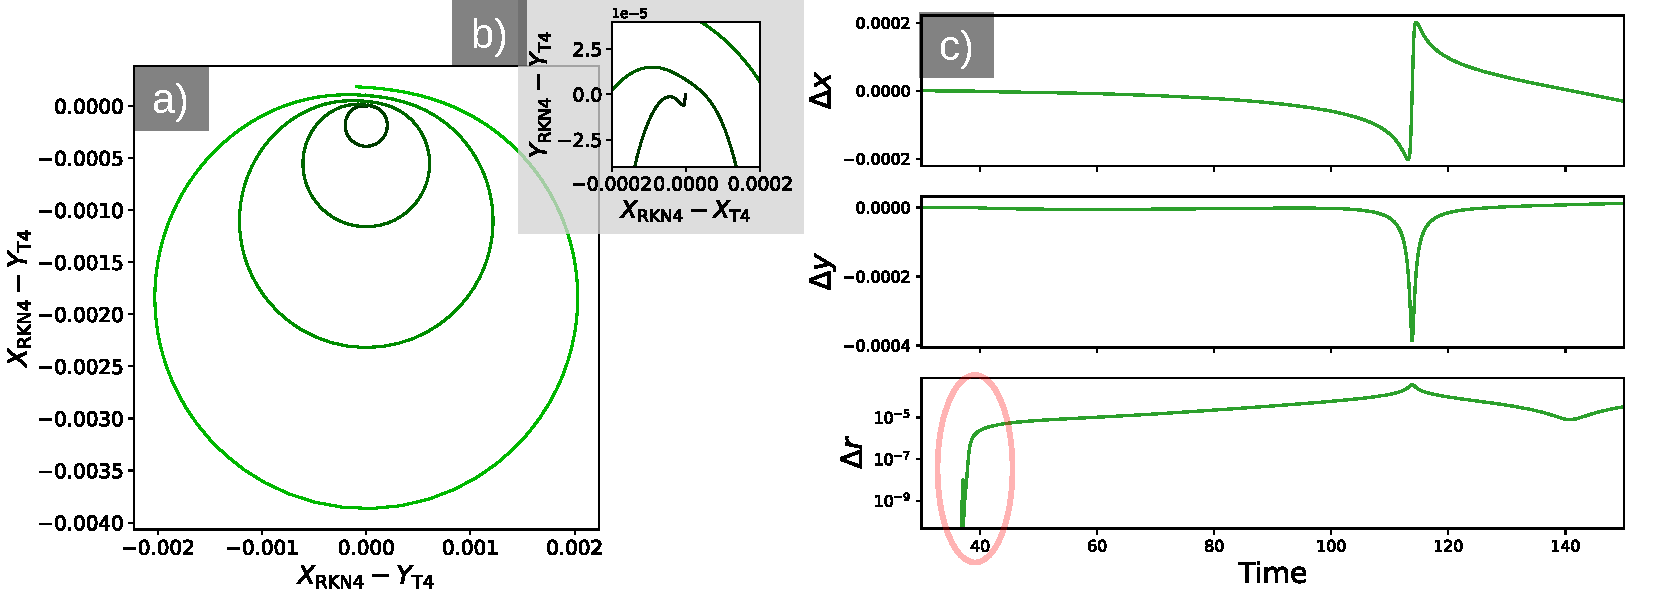
\includegraphics[width=1.0\linewidth]{diagrams/p3_orbitDifferences}
		\caption{The difference of the orbit positions at each time step is plotted. In plot (a) the spatial coordinates are shown with color gradient changing from black at $t=0$ to green at $t=5P$. In plot (b) the plot area is zoomed to the origin to show that the deviations between the two orbits is initially quite small. In plot (c) the time dependence of the spatial coordinate differences are shown. Additionally the value of $\Delta r^2 = \Delta x^2 + \Delta y^2$ is plotted on a log-y scale. Highlighted in with a red oval is the rapid increase in the deviations from the two trajectories.}
		\label{fig:p3orbitdifferences}
	\end{figure}
	
	For nearly one half of the orbital period, the two trajectories agree to the entire machine precision of the simulation. The first deviation between the two orbits appears as seemingly round-off error between two different evaluations of the same function. This slight error initially grows rapidly (see the highlighted portion of Figure \ref{fig:p3orbitdifferences} (c)), but then is seen to grow essentially linearly after each orbit (see Figure \ref{fig:p3orbitdifferences} (a)), indicating that the two methods must be of the same order in error. From this behavior, we can conclude that the \underline{two methods are the same}, differing only in the steps of evaluation.
	
	These slight differences resulting from the method of execution can be thought of as analogous to the evaluation of polynomials on a finite-sized floating point system. The precision resulting from evaluation of the expanded polynomial $a_n x^n + a_{n-1} x^{n-1} \ldots + a_1 x + a_0$ is not the same precision resulting from the evaluation of the factored polynomial $(x-b_n)(x-b_{n-1})\ldots(x-b_1)b_0$ even if the two functions are mathematically identical. In the case of comparing two iterative methods, these slight differences in computation are amplified in subsequent steps of the algorithm.
	
	Attached at the end of the document is the code which executes these simulations. It can be seen that there is much greater ease in defining the procedure implied by $\hat{T}_4$ than there is for the RKN4 algorithm. This cleanliness of implementation is essentially forced on the simulation architect, as the execution of the operator $\hat{T}_4$ is already broken down into smaller operations which are conveniently packaged into a subroutine.
	
	The structure of the operator representing the RKN4 algorithm (containing an addition operation) does not allow a convenient representation in terms of an algorithm Hamiltonian. This can be regarded as a serious disadvantage because obtaining the algorithm Hamiltonian allows for a powerful method of error quantification and correction.
	
	\section{4th order Forest-Ruth algorithm and energy fluctuations}
	In this section we investigate energy fluctuations between the 4th order Runge-Kutta-Nystrom (RKN4) algorithm and the 4th order Forest-Ruth algorithm for the same initial conditions as the previous section.
	
	The 4th order Forest-Ruth algorithm can be defined by the following operator
	\begin{equation}
		\hat{T}^{(4)}_\mathrm{PV} = \hat{T}^{(2)}_\mathrm{PV}(\epsilon)
		\hat{T}^{(2)}_\mathrm{PV}(-s\epsilon)
		\hat{T}^{(2)}_\mathrm{PV}(\epsilon)
	\end{equation}
	This operator structure strongly reflects how the method was implemented in the simulation code, using position-Verlet subroutines to accomplish a single 4th order step.
	
	This operator can also be written in exponential form (see Appendix), which shows that the method approaches the exact time evolution operator as $\epsilon^4$ when the we choose $s=2^{1/3}$. This transformation also forces us to scale the time step to be $\Delta t = \epsilon(2-2^{1/3})$.
	
	For the same initial conditions previously discussed, we plot the resulting energy fluctuations for 15 orbital periods of the two algorithms at three different time steps: $\Delta t / P = 1000, 2000, 4000$. The resulting energy fluctuations are shown in Figure \ref{fig:p4energyfluctuations}.
	
	\begin{figure}[H]
		\centering
		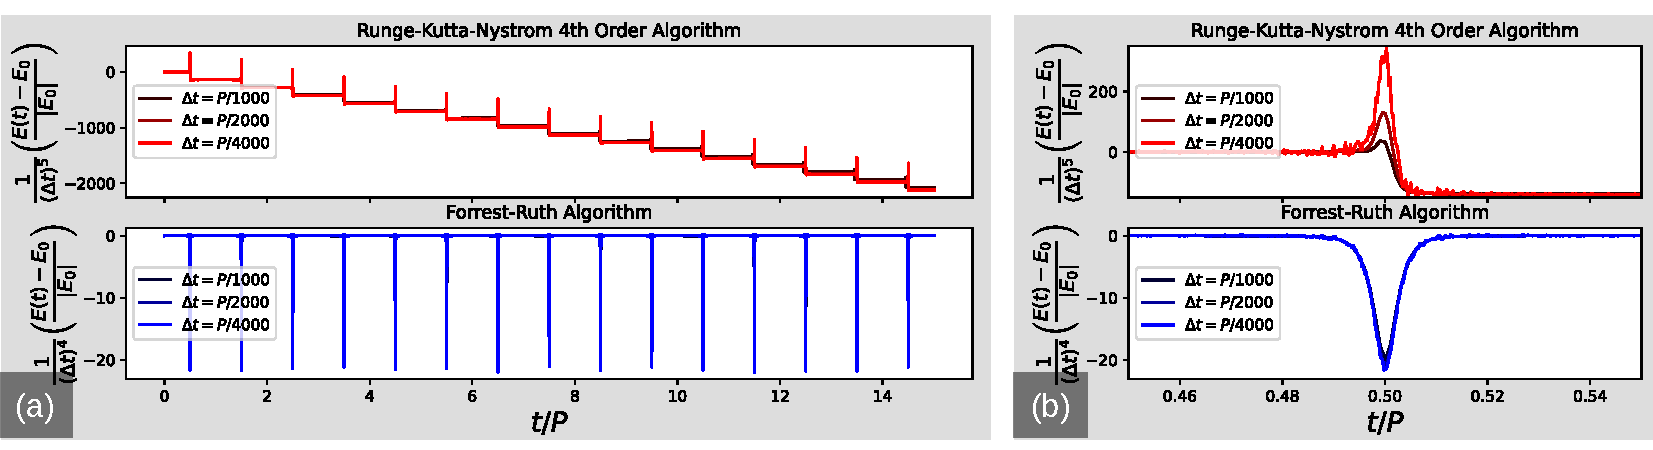
\includegraphics[width=1.0\linewidth]{diagrams/p4_energyFluctuations}
		\caption{Energy Fluctuations. In graph (a) we see the energy of the RKN4 method (upper red) decreasing over many periods, whereas the symplectic method (lower blue) is stable in regard to drift over many orbital periods of the total system energy despite having significantly larger fluctuations.}
		\label{fig:p4energyfluctuations}
	\end{figure}
	
	It can be seen that the RKN4 method does not exhibit long-term stability of the total system energy, whereas the symplectic method seems to preserve the system energy on average seemingly indefinitely. The magnitude of energy fluctuations in the symplectic algorithm are significantly larger than those of the RKN4 method. It would take many orbital periods for the energy fluctuation of the RKN4 algorithm to "walk" to the same magnitude of discrepancy as the symplectic method, but by this time the predicted orbital geometry is completely different.
	
	Scaling the energy fluctuations by $1/\Delta t^N$ allows us to see that the rate of energy "walk-off" in the RK4 method is changing with $\Delta t^5$. However, the magnitude of the energy spike near closest approach seems to scale as $\Delta t^4$ (not shown on this scale), which is consistent with this being a fourth order method. We see this same scaling relation in the magnitude of the brief energy spikes occurring in the $\hat{T}^{(4)}_\mathrm{PV}$ simulated system, which is consistent with this operator coinciding with the exact evolution operator to fourth order in $\Delta t$.
	
	\section{Orbital Precession}
	For this section we use the same simulation data generated in the last section, but instead we analyze how the algorithm evolution affects the Laplace-Runge-Lenz vector. This vector is normally conserved for a particle orbiting a central inverse square force, as in Newtonian gravitation, and gives information about the orientation of the ellipse that would be traced by the exact solution of the trajectory under the action of such a force. This vector $\mathbf{A}$ is defined by
	\begin{equation}
		\mathbf{A} = \mathbf{v}\times \mathbf{L} - \hat{\mathbf{r}}
	\end{equation}
	This vector always lies in the plane of the orbit, and is oriented parallel to the semi-major axis. For the intial value problem that we have previously outlined, the exact value of $\mathbf{A}$ lies along the $x$-axis. With this coordinate orientation, we can calculate rotation of this vector arising from the algorithm action as the rotation angle
	\begin{equation}
		\Delta \theta = \tan^{-1}\frac{A_y}{A_x}
	\end{equation}
	With this definition, we plot the rotation angle $\Delta \theta$ over time for the same simulation data generated in the previous part. In order to investigate the scaling relation of this quantity against a changing time-step $\Delta t$, we plot the quantity $\Delta \theta/(\Delta t)^4$ for several values of the time-step.
	\begin{figure}[H]
		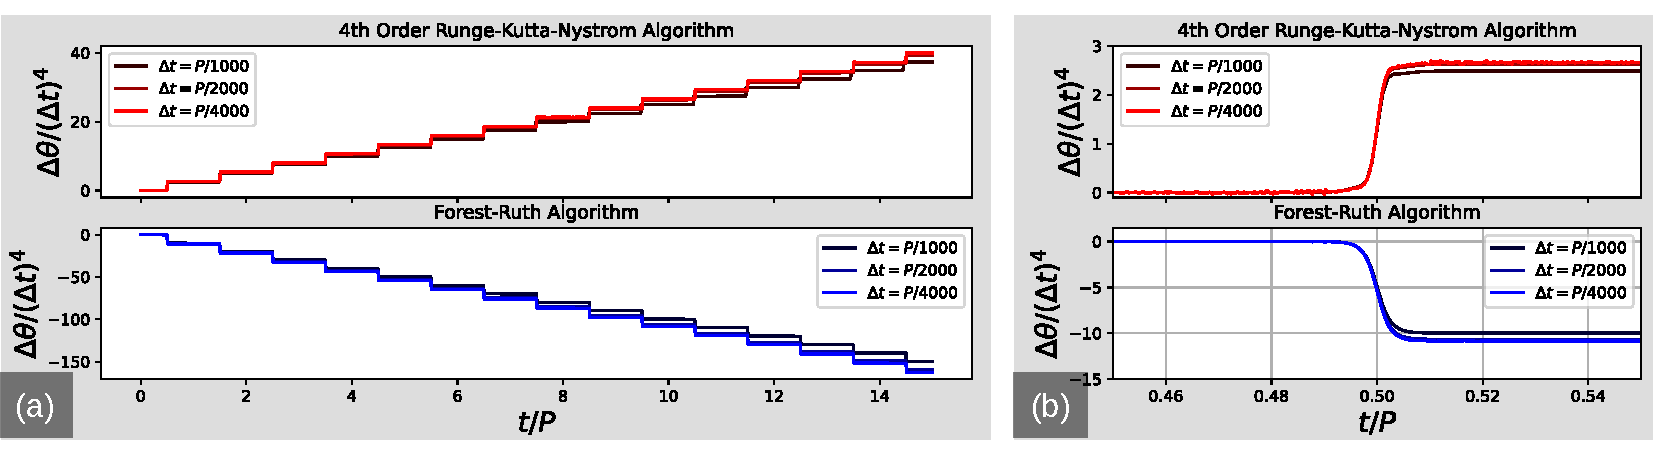
\includegraphics[width=1.0\linewidth]{diagrams/p5_precession}
		\caption{Orbital precession.}
		\label{fig:p5precession}
	\end{figure}
	Under this scaling, the plots can be seen to nearly trace over one another. Therefore it can be seen from the plots of precession angle that both the Forest-Ruth and RKN4 algorithms have a precession rate decreasing as $(\Delta t)^4$.
	
	\section{Estimation of Perihelion Advance}
	It is in principle possible to calculate the rate of precession in terms of just the eccentricity $e$ of the exact orbit, and the time step $\Delta t$ for any algorithm which can be written as a product of displacement operators.
	
	In this section we make a switch in the velocity variable $\mathbf{v}\rightarrow\mathbf{p}$. Although these quantities are numerically equal in our dimensionless units, we do this in order to ensure clarity of notation. The Hamiltonian of the exact problem which we are solving is given by
	\begin{equation}
		H(\mathbf{r}, \mathbf{p}) = T(\mathbf{p}) + V(\mathbf{r}) = \frac{1}{2}\mathbf{p}\cdot\mathbf{p} - \frac{1}{|\mathbf{r}|}
	\end{equation}
	
	We can construct a form of the exact evolution operator which resembles those of the algorithm evolution operators considered earlier. The exact evolution operator of the system Hamiltonian $H$ can be written
	\begin{align}
		e^{\hat{H}} &= e^{\epsilon(\hat{T} + \hat{V})} \\
		&= e^{\epsilon\hat{T}} e^{\epsilon\hat{V}} e^{-\frac{\epsilon^2}{2}[\hat{T},\hat{V}]} e^{-\frac{\epsilon^3}{6}(2[\hat{V},[\hat{T},\hat{V}]] + [\hat{T},[\hat{T},\hat{V}]])} 
		\ldots
	\end{align}
	Where $\hat{H}$ is the operator corresponding to the system Hamiltonian $H$. This expansion is known as the Zassenhaus formula. We include it here to illustrate that it is natural to construct an algorithm which is a product of carefully chosen displacement operators which resemble in low order the above expression.
	
	The above expansion of the exact evolution operator by itself is not very useful in the present case, as it does not reflect the fact that there is time-reversal symmetry in our problem (no energy dissipation). This form of the evolution operator must preserve this symmetry, and therefore terms of even order in $\epsilon$ must be zero. This is evident in lower order terms, such as the $[\hat{T}, \hat{V}]$ term which corresponds to a dissipative force proportional to $\mathbf{p}\cdot\mathbf{v}$.
	
	Instead we seek a time evolution operator which approximates the time exact time evolution operator in the form
	\begin{align}
		e^{\epsilon(\hat{T} + \hat{V})} \approxeq \prod_{i=1}^{N} \exp\Big({t_i \epsilon\hat{T}}\Big) \exp\Big({v_i\epsilon\hat{V}}\Big) = e^{\hat{H}_A}
	\end{align}
	
	We have seen previously the advantages of choosing a symplectic algorithm, and how this property can be obtained by ensuring that our resulting algorithm is time-reversal symmetric. In such a manner, we choose the coefficients $t_i$ and $v_i$ to be symmetric, that is $t_i = t_{N-i}$ and $v_i = v_{N-i}$. The operator of such an algorithm would then read
	
	\begin{align}
		e^{\epsilon(\hat{T} + \hat{V})} &\approxeq e^{\epsilon t_0\hat{T}} e^{\epsilon v_0\hat{V}}
		e^{\epsilon t_1\hat{T}} e^{\epsilon v_1\hat{V}} \ldots
		e^{\epsilon t_1\hat{T}} e^{\epsilon v_1\hat{V}}
		e^{\epsilon t_0\hat{T}} e^{\epsilon v_0\hat{V}} \\
		&=
		(1+t_0\epsilon \hat{T} + \cdots)
		(1+v_0\epsilon \hat{V} + \cdots) \ldots
		(1+t_N\epsilon \hat{T} + \cdots)
		(1+v_N\epsilon \hat{V} + \cdots)  \\
		&=
		1 + \epsilon\left(\sum_{i=0}^{N} t_i\right)\hat{T} + \epsilon\left(\sum_{i=0}^{N} v_i\right)\hat{V} + \cdots
	\end{align}
	The sums enclosed in the parentheses are enforced to be equal to one to ensure that agreement with the exact time evolution operator in lowest order of the timestep $\epsilon$. This constraint along with the symmetry requirement define all possible symplectic algorithms.
	
	In order to use the above formulation for error quantification, it is useful to evaluate the approximate form of the algorithm Hamiltonian $\hat{H}_A$ for the particular choice of $t_i$ and $v_i$ which define the algorithm. While having nothing to do with the real physics of the original problem, this modified Hamiltonian allows our procedure to represent an exact evolution operator for which we can use the tools of real physics to analyze.
	
	The basic approach is as such; calculate the algorithm Hamiltonian by converting the operator commutator expansion into a function expanded in Poisson brackets. The algorithm Hamiltonian represents the problem Hamiltonian plus a small perturbative potential. The gradient of this perturbing potential gives us the perturbative force $f(r)$, which for the scope of this discussion will only dependent on distance to coordinate origin. The $\mathbf{A}$ vector changes as
	
	\begin{equation}
		\mathbf{\dot{A}} = \mathbf{\Omega} \times \mathbf{A}
	\end{equation}
	
	It can be shown that for our symmetric force, the rotation vector $\mathbf{\Omega} = -f(r)\frac{L}{e}\cos \theta \mathbf{\hat{L}}$ can be calculated to give a rotation angle of
	
	\begin{equation}
		\Delta \theta = \frac{1}{e}\int_{0}^{2\pi}(-f(r)r^2)\cos\theta d\theta
	\end{equation}
	
	\subsection{Precession of the Cromer and Newton Methods}
	In the Appendix, we have the following algorithm Hamiltonian for the two methods.
	\begin{equation}
		H_A = T(\mathbf{p}) + V(\mathbf{r}) \pm \underbrace{\epsilon\{T,V\}}_{\text{Periodic Energy Error}} + \underbrace{\frac{\epsilon^2}{12}\Big(\{TVV\} - \{TVT\}\Big)}_{\text{Orbital Precession}}  + O(e^4)
	\end{equation}
	These Poisson brackets can be evaluated (see Appendix) as
	\begin{align}
		\{T,V\} &= - p_iV_i \\
		\{VTV\} &= -V_iV_i \\
		\{TTV\} &= p_i V_{ij} p_j
	\end{align}
	For the case of a inverse square law force (Kepler problem), these brackets read
	\begin{align}
		\{V,T\} &= \frac{\mathbf{r}\cdot \mathbf{p}}{r^3} \\
		\{VTV\} &= \frac{-1}{r^4} \\
		\{TTV\} &= \frac{-3}{r^5}\big(\mathbf{r} \cdot \mathbf{p}\big)
	\end{align}
	These terms act as perturbing Hamiltonians to the original problem. This causes a violation of Bertrand's theorem strongest near the center of force, and an associated precession of the orbit.
	
	In order to save space at this point, we regress to symmetry arguments. We observed that the Newton and Cromer methods conserve energy on average, therefore dissipation terms proportional to $\mathbf{r}\cdot\mathbf{p}$ must average out. Because the precession always marches on in the same direction the precession cannot be due to these terms, as they must have opposite signs on opposite halves of the periodic trajectory. Therefore the error term in the algorithm Hamiltonian proportional to $1/r^4$ must be responsible for the precession. This corresponds to a fictitious force proportional to $-4/r^5$ which is the effect of the stepping algorithm.
	
	Under the action of a perturbation force $f(r) = -1/r^n$, the precession of the Laplace-Runge-Lenz vector can be calculated from
	\begin{align*}
		\Delta \theta &= \frac{1}{e}\int_{0}^{2\pi}(-f(r)r^2)\cos\theta d\theta \\
		&= \frac{1}{e}\int_{0}^{2\pi}\frac{\cos\theta d\theta}{r^{N-2}}
	\end{align*}
	We make the simplifying assumption that the trajectory of the particle is somewhat near the exact orbit ellipse, allowing us to make use of the parameterization
	\begin{equation}
		r(\theta) = \frac{p}{1-e\cos\theta}
	\end{equation}
	\begin{equation}
		\frac{1}{r} = \frac{1}{\mathcal{P}}(1+ e\cos\theta)\;\;\;\;;\;\;\;\; \mathcal{P} = a(1-e^2)
	\end{equation}
	Per orbital period, we obtain the value for the total precession angle of the LRL vector
	\begin{align*}
		\Delta \theta &= \frac{1}{e}\int_{0}^{2\pi}(-f(r)r^2) \\
		&= \frac{1}{e\mathcal{P}^{N-2}}\int_{0}^{2\pi} (1+e\cos\theta)^{N-2} \cos\theta d\theta
	\end{align*}
	Using the Newton or Cromer method introduces a fictitious force going as $1/r^5$, therefore we have in the above relation $N=5$. For this particular value, the integral in the above relation becomes
	\begin{align}
		\frac{1}{e}\int_{0}^{2\pi} (1+e\cos\theta)^{3} \cos\theta d\theta = 3\pi\Big(1 + \frac{1}{4}e^2\Big)
	\end{align}
	
	For the simulation in Project 1, with $\Delta t = 500/P$ we obtain a rotation of the obit ellipse during each half-period of
	\begin{equation}
		\Delta \theta_\text{1/2} = \frac{1}{2}4\frac{1}{12}\;(\Delta t)^2 3\pi \Big(1+\frac{e^2}{4}\Big) = (\Delta t)^2 \frac{\pi}{2}\Big(1+\frac{e^2}{4}\Big) \approx 0.0482
	\end{equation}
	The first factor of $1/2$ comes from the fact that we want the precession during one-half orbit. The second factor of $4$ arose from the differentiation of the $1/r^4$ error term of the algorithm Hamiltonian to obtain the perturbation force. The third factor of $1/12$ arose from our commutator expansion of the algorithm operator. The resulting value is marked in the proceeding Figure, along-side the angle of the LRL vector directly computed from the resulting orbit trajectory.
	
	From the above relation, we can see that the precession of the orbit ellipse is first order in $\Delta t$
	\begin{align*}
		\Delta \theta &\sim (\Delta t)^2 \\
		\frac{\Delta \theta}{\Delta t} &\sim \Delta t
	\end{align*}
	
	\begin{figure}[H]
		\centering
		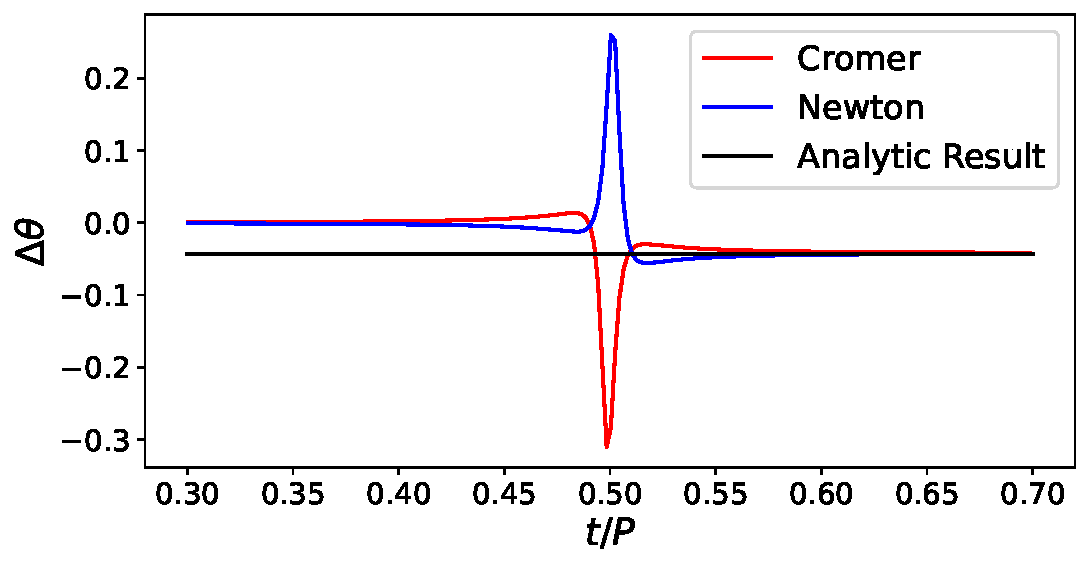
\includegraphics[width=1.0\linewidth]{diagrams/precessionCalc}
		\caption{Precession angle compared to analytic result.}
		\label{fig:precessioncalc}
	\end{figure}
	
	\section{Appendix}
	Some of the relations contained in this section were covered in class, but I include them for completeness.
	\subsection{Baker-Cambell-Hausdorf Formula}
	\begin{equation}
		e^{\epsilon(\hat{T}+\hat{V})} = \exp\Big( \hat{T} + \hat{V} + \frac{1}{2}[\hat{T},\hat{V}] + \cdots\Big) 
	\end{equation}
	We will make heavy use of this expression. In order to assist our efforts, we use a computer algebra system to aid our efforts. This is attached at the end of this document.
	
	\subsection{Commutator Expansions}
	\subsubsection{Cromer Method}
	\begin{align}
		\hat{T}^{(1)}_\mathrm{a} &= e^{\epsilon \hat{V}} e^{\epsilon \hat{T}} \\
		&= \exp\Bigg(\epsilon\hat{T} + \epsilon\hat{V} - \frac{\epsilon^2}{2}[\hat{T},\hat{V}] + \frac{\epsilon^3}{12}\Big([TVV] - [TVT]\Big)  + O(e^4) \Bigg)
	\end{align}
	\subsubsection{Newton Method}
	\begin{align}
		\hat{T}^{(1)}_\mathrm{b} &= e^{\epsilon \hat{T}} e^{\epsilon \hat{V}} \\
		&= \exp\Bigg(\epsilon\hat{T} + \epsilon\hat{V} + \frac{\epsilon^2}{2}[\hat{T},\hat{V}] + \frac{\epsilon^3}{12}\Big([TVV] - [TVT]\Big)  + O(e^4) \Bigg)
	\end{align}
	
	We see that the two first order methods have opposite signs of the lowest order term $\epsilon^2$. We can now formally account for the opposite-going behavior of the energy fluctuations we observed in the last project.
	
	The two fundamental sequential stepping operators give an algorithm Hamiltonian of the form
	\begin{equation}
		H_A = T(\mathbf{p}) + V(\mathbf{r}) \pm \underbrace{\epsilon\{T,V\}}_{\text{Periodic Energy Error}} + \underbrace{\frac{\epsilon^2}{12}\Big(\{TVV\} - \{TVT\}\Big)}_{\text{Orbital Precession}}  + O(e^4)
	\end{equation}
	The underlined terms have been identified by the following observations. In the last project, we observed in the first order simulations a periodic error which was of approximately opposite sign for the two methods. This energy error was always averaging to zero, yet the orbit ellipse was observed to precess in the same direction. Therefore we argue that the $\epsilon\{T,V\}$ term must average to zero during the course of an orbit, and cannot affect the ellipse orientation otherwise a reversal would be observed upon interchange of the two methods. To lowest order $\epsilon^2$, we must have that the precession of the orbital ellipse is entirely determined by the double-Poisson brackets in the parentheses. Because this term is identical for both first order methods, we identify the precession direction and rate as being the same for both first order methods.
	
	We note that the higher-order symplectic methods investigated here seem to have a similar identification.
	\subsubsection{Position-Verlet Method}
	\begin{align}
		\hat{T}^{(2)}_\mathrm{PV}	&= e^{\epsilon \hat{T}/2}e^{\epsilon \hat{V}} e^{\epsilon \hat{T}/2} \\
		&= \hat{T}^{(1)}_\mathrm{b}\left(\frac{\epsilon}{2}\right) \hat{T}^{(1)}_\mathrm{a}\left(\frac{\epsilon}{2}\right) \\
		%&= e^{\epsilon \hat{T}/2} \exp\Big(\frac{\epsilon}{2}\hat{T} + \epsilon\hat{V} - \frac{\epsilon^2}{2}[\hat{T},\hat{V}]\Big) \\
		%&= \exp\Big(\epsilon\hat{T} + \epsilon\hat{V} + \frac{\epsilon^3}{16}[\hat{T},[\hat{V},\hat{T}]]\Big) \\
		&= \exp\Bigg(\epsilon\hat{T} + \epsilon\hat{V} + \frac{\epsilon^3}{24}\Big([TVT] + 2[VVT]\Big) + \frac{\epsilon^4}{384}\Big([VTVT] - [TVVT]\Big) + O(e^5) \Bigg) \\
	\end{align}
	We observe second order convergence in the time-step $\epsilon$ for the position-Verlet method as well as the velocity-Verlet method below.
	\subsubsection{Velocity-Verlet Method}
	\begin{align}
		\hat{T}^{(2)}_\mathrm{VV}	&= e^{\epsilon \hat{V}/2}e^{\epsilon \hat{T}} e^{\epsilon \hat{V}/2} \\
		&= \hat{T}^{(1)}_\mathrm{a}\left(\frac{\epsilon}{2}\right) \hat{T}^{(1)}_\mathrm{b}\left(\frac{\epsilon}{2}\right) \\
		&= \exp\Bigg(\epsilon\hat{T} + \epsilon\hat{V} - \frac{\epsilon^3}{24}\Big(2[TVT] + [VVT]\Big) + \frac{\epsilon^4}{384}\Big([VTVT] - [TVVT]\Big) + O(e^5) \Bigg)
	\end{align}
	The two fundamental second order symplectic methods have the algorithm Hamiltonian
	\begin{equation}
		H_A = T(\mathbf{p}) + V(\mathbf{r}) \pm \underbrace{\frac{\epsilon^2}{24}\Big(\ldots\Big)}_{\text{Periodic Energy Error}} + \underbrace{\frac{\epsilon^3}{384}\Big(\{VTVT\} - \{TVVT\}\Big)}_{\text{Orbital Precession}}  + O(e^4)
	\end{equation}
	\subsubsection{Forest-Ruth Algorithm}
	\begin{align}
		\hat{T}^{(4)}_\mathrm{PV} &= \hat{T}^{(2)}_\mathrm{PV}(\epsilon)\hat{T}^{(2)}_\mathrm{PV}(-s\epsilon)\hat{T}^{(2)}_\mathrm{PV}(\epsilon) \\
		&= \exp\Bigg(\epsilon(2-2^{1/3})( \hat{T} + \hat{V}) + (1+2^{1/3})\frac{\epsilon^4}{192}\Big([VTVT] - [TVVT]\Big) + O(\epsilon^5)\Bigg)\\
	\end{align}
	We see from the above operator expansion that we are naturally lead to the substitution for the time step $\Delta t = \epsilon(2-2^{1/3})$. The value of $s=2^{1/3}$ allows the $\epsilon^3$ term to vanish.
	
	\subsection{Poisson Bracket Expansions}
	The time dependence of any dynamical variable $W(r_i, p_i)$ which can be expressed solely in terms of the fundamental coordinates $r_i$ and $p_i$ can be expressed as
	\begin{align}
		\frac{dW}{dt} &= \frac{\partial W}{\partial r_i} \frac{\partial r_i}{\partial t} + \frac{\partial W}{\partial p_i} \frac{\partial p_i}{\partial t} \\
		&= \frac{\partial W}{\partial r_i} \frac{\partial H}{\partial p_i} - \frac{\partial W}{\partial p_i} \frac{\partial H}{\partial r_i }	\\
		&= \{W,H\}
	\end{align}
	Any other dynamical variables $A(r_i, p_i)$  and $B(r_i, p_i)$ have similar time dependencies, and this underlying relation to the fundamental coordinates allows us to directly relate those two quantities using the Poisson bracket. For this purpose we say that the operator $\hat{A}$ corresponds to the dynamical variable $A(r_i, p_i)$, and the operator $\hat{B}$ corresponds to the dynamical variable $B(r_i, p_i)$. The action of operator $\hat{A}$ on $B(r_i, p_i)$, and vice versa, is then defined by the Poisson brackets
	\begin{align}
		\hat{A} B &= \{B, A\} \\
		\hat{B} A &= \{A, B\}
	\end{align}
	\subsubsection{First Order}
	We recall the dependence of the kinetic energy $T$ and potential energy $V$ on the generalized coordinates
	\begin{align*}
		T &= \frac{1}{2}p_i^2 \\
		V &= V\Big(r(r_i)\Big)\;\;\;;\;\;\;r(r_i)=(r_i r_i)^{1/2}
	\end{align*}
	Keeping these in mind, we can see the great simplifications which occur in the expressions of the Poisson brackets.
	\begin{align}
		\{T,V\} &= \frac{\partial T}{\partial r_i} \cancel{\frac{\partial V}{\partial p_i}} - \frac{\partial T}{\partial p_i} \frac{\partial V}{\partial r_i } \\
		&= - \frac{\partial T}{\partial p_i} \frac{\partial V}{\partial r_i } \\
		&= -p_i\frac{\partial V}{\partial r_i } = -p_i V_i
	\end{align}
	This Poisson bracket defines the action of operator $\hat{V}$ on $T$. Because the Poisson bracket is anti-commutative, we can also express the action of $\hat{T}$ on $V$.
	\begin{align}
		\hat{V}T &= -p_i V_i \\
		\hat{T}V &=  p_i V_i
	\end{align}
	Collecting so far, we have
	\begin{equation}
		\boxed{\{V,T\} = p_i V_i}
	\end{equation}
	\begin{equation}
		\boxed{\{T,V\} = -p_i V_i}
	\end{equation}
	\subsubsection{Second Order}
	Recalling the definition of the operators $\hat{T}$ and $\hat{V}$
	\begin{align}
		\hat{T} &= p_i \frac{\partial}{\partial r_i}  &&= p_i\partial^{(r)}_i \\
		\hat{V} &= -V_i \frac{\partial}{\partial p_i} &&= -V_i\partial^{(p)}_i
	\end{align}
	The above definition is consistent with what we introduced in Part 1 but for a spherically symmetric force function. That is, we have in vector notation the relation $\mathbf{a}(\mathbf{r}) = - \mathbf{\nabla} V(r)$. We also make note of the slightly confusing subscript notation. The subscript $V_i$ refers to the derivative $\partial V/\partial r_i$, whereas the subscripts $p_i$ and $r_i$ refer to the corresponding $x$, $y$, or $z$ coordinate.
	
	With this in mind, we have for the first set of nested brackets
	\begin{align*}
		\{TTV\} &= \{T, \{T,V\}\} \\
		&= \{T, -p_iV_i\} \\
		&= \{p_i V_i, T\} \\
		&= \hat{T}\Big[p_i V_i\Big] \\
		&= p_j\partial^{(r)}_j\Big[p_i V_i\Big] \\
		&= p_i p_j\partial^{(r)}_j\Big[V_i\Big] \\
		&= p_j p_i V_{ij} \\
	\end{align*}
	\begin{align*}
		\{VTV\} &= \{V, \{T,V\}\} \\
		&= \{V, -p_iV_i\} \\
		&= \{p_i V_i, V\} \\
		&= \hat{V}\Big[p_i V_i\Big] \\
		&= -V_j\partial^{(p)}_j\Big[p_i V_i\Big] \\
		&= -V_j V_i \delta_{ij} \\
		&= -V_iV_i \\
	\end{align*}
	Collecting the nested brackets, we have
	\begin{equation}
		\boxed{	\{TTV\} = p_i V_{ij} p_j}
	\end{equation}
	\begin{equation}
		\boxed{	\{VTV\} = -V_iV_i }
	\end{equation}
	
	\subsection{Spatial Derivatives of Radial Potential}
	
	For a radial potential, we can express the entire spatial dependence using a scalar function of the position vector magnitude
	\begin{equation}
		V(\mathbf{r}) = V(r)\;\;\;;\;\;\; r = (\mathbf{r}\cdot\mathbf{r})^{1/2}
	\end{equation}
	Differentiation of this scalar function is straightforward, but then we must take into account how the position vector magnitude changes
	\begin{align}
		\mathbf{\nabla}\left[V(\mathbf{r})\right] &= \mathbf{\nabla}\left[V(r)\right] \nonumber \\
		&= V'(r)\mathbf{\nabla}\left[r\right]
	\end{align}
	For details of such calculations, the reader is referred to the proceeding subsection.
	
	We now proceed with the evaluation of derivatives
	
	\begin{align}
		\partial_i [V(r)] &= V'(r)\partial_i[r] \\
		&= V'(r)\mathbf{\hat{r}}_i
	\end{align}
	\begin{equation}
		\boxed{V_i = V'(r)\mathbf{\hat{r}}_i}
	\end{equation}
	
	All combinations of second derivatives can be evaluated as
	\begin{align}
		V_{ij} &= \partial_j[V'(r)\mathbf{\hat{r}}_i] \\
		&= V''(r)\mathbf{\hat{r}}_i \mathbf{\hat{r}}_j + \underbrace{\frac{V'(r)}{r}}_{\textcolor{blue}{\equiv U(r)}}\left[\delta_{ij} - \mathbf{\hat{r}}_i \mathbf{\hat{r}}_j\right]
	\end{align}
	If we now define the function $U(r)$ as the following
	\begin{equation}
		U(r) = \frac{V'(r)}{r}
	\end{equation}
	Then the second spatial derivatives of the potential can be written as
	\begin{equation}
		\boxed{V_{ij} = U \delta_{ij} +\left(V'' - U\right)}
	\end{equation}
	We also make note of the first derivative of the scalar function $U(r)$
	\begin{align}
		U'(r) &= \frac{V''(r)}{r} - \frac{V'(r)}{r^2} \\
		U'	  &= \frac{V''}{r} - \frac{U}{r}
	\end{align}
	\begin{equation}
		\boxed{U' = (V'' - U)/r}
	\end{equation}
	
	Proceeding with the third derivatives in the spatial coordinates
	\begin{align}
		V_{ijk} &= \partial_k \Big[ U \delta_{ij} +\left(V'' - U\right) \Big] \\
		&= U'\mathbf{\hat{r}}_i \delta_{ij} + \left(V''' - U'\right) \mathbf{\hat{r}}_i \mathbf{\hat{r}}_j \mathbf{\hat{r}}_k + (V'' - U)\partial_k[\mathbf{\hat{r}}_i \mathbf{\hat{r}}_j] \\
		&= U'\mathbf{\hat{r}}_i \delta_{ij} + \left(V''' - U'\right) \mathbf{\hat{r}}_i \mathbf{\hat{r}}_j \mathbf{\hat{r}}_k + \underbrace{\frac{(V'' - U)}{r}}_{\textcolor{blue}{=U'(r)}}\Big(\mathbf{\hat{r}}_i \delta_{ij} + \mathbf{\hat{r}}_j \delta_{ik} - 2\mathbf{\hat{r}}_i \mathbf{\hat{r}}_j \mathbf{\hat{r}}_k \mathbf{\hat{r}}_j\Big) \\
	\end{align}
	\begin{equation}
		\boxed{V_{ijk} = U'\Big(\mathbf{\hat{r}}_i \delta_{jk} + \mathbf{\hat{r}}_j \delta_{ik} + \mathbf{\hat{r}}_k \delta_{ij} \Big) + (V''' - 3U')\mathbf{\hat{r}}_i \mathbf{\hat{r}}_j \mathbf{\hat{r}}_k}
	\end{equation}
	\subsubsection{Spatial Derivatives of the Vector Magnitude $r = (\mathbf{r}\cdot\mathbf{r})^{1/2}$}
	We wish to evaluate the partial derivatives of the function $|r| = (x^2 + y^2 + z^2)^{1/2}$. We look at the partial derivative in $x$ coordinate
	\begin{equation}
		\frac{\partial |r|}{\partial x} = \frac{x}{\left(x^2 + y^2 + z^2\right)^{1/2}} = \frac{x}{r} = \mathbf{\hat{r}}_x
	\end{equation}
	The symmetry of the function $|r|$ in all the coordinates should be observed. Had we differentiated with respect to the $i^\mathrm{th}$ coordinate $x_i$ then we would obtain
	\begin{equation}
		\boxed{\partial_i |r| = \frac{x_i}{r} \equiv \mathbf{\hat{r}}_i}
	\end{equation}
	
	For the sake of notational compactness, we now switch to Einstein-summation. We proceed to evaluate further derivatives of the vector magnitude function
	\begin{align}
		\partial_j\left[ \mathbf{\hat{r}}_i \right] &= \partial_j\left[\frac{x_i}{r}\right] \\
		&= \frac{\delta_{ij}}{r} - \frac{x_i}{r^2}\partial_j[r] \\
		&= \frac{\delta_{ij}}{r} - \frac{x_i}{r^2}\frac{x_j}{r}
	\end{align}
	\begin{equation}
		\boxed{\partial_j\left[ \mathbf{\hat{r}}_i \right] =  \frac{\delta_{ij}}{r} - \frac{\mathbf{\hat{r}}_i \mathbf{\hat{r}}_j}{r}}
	\end{equation}
	
	We also encounter derivatives of type
	\begin{align}
		\partial_k[\mathbf{\hat{r}}_i \mathbf{\hat{r}}_j] &= \mathbf{\hat{r}}_i \partial_k[\mathbf{\hat{r}}_j] + \partial_k [\mathbf{\hat{r}}_i] \mathbf{\hat{r}}_j \\
		&= \frac{\mathbf{\hat{r}}_i}{r} \Big( \delta_{jk} - \mathbf{\hat{r}}_j \mathbf{\hat{r}}_k \Big)  + \Big( \delta_{ik} - \mathbf{\hat{r}}_i \mathbf{\hat{r}}_k \Big) \frac{\mathbf{\hat{r}}_j}{r} \\
		&= \frac{1}{r}\Big(\mathbf{\hat{r}}_i \delta_{ij} + \mathbf{\hat{r}}_j \delta_{ik} - 2\mathbf{\hat{r}}_i \mathbf{\hat{r}}_j \mathbf{\hat{r}}_k \mathbf{\hat{r}}_j\Big)
	\end{align}
	\begin{equation}
		\boxed{\partial_k[\mathbf{\hat{r}}_i \mathbf{\hat{r}}_j] = \frac{1}{r}\Big(\mathbf{\hat{r}}_i \delta_{ij} + \mathbf{\hat{r}}_j \delta_{ik} - 2\mathbf{\hat{r}}_i \mathbf{\hat{r}}_j \mathbf{\hat{r}}_k \mathbf{\hat{r}}_j\Big)}
	\end{equation}
	
	\subsection{Evaluation of Algorithm Hamiltonians}
	The earlier forms of the algorithm Hamiltonians were not particularly useful in that they were not directly expressed in quantities which were accessible to a simulator program. To make these more useful, we must convert the Poisson brackets into explicit expressions of the generalized coordinates.
	
	\begin{align}
		\{V,T\} &= p_i V_i \\
		&= p_i V'(r)\mathbf{\hat{r}}_i \\
	\end{align}
	We can conveniently express this quantity in vector notation as
	\begin{equation}
		\boxed{\{V,T\} = (\mathbf{\hat{r}} \cdot p)V'(r)}
	\end{equation}
	We see that this term includes a mixing of the momentum and position coordinates into the algorithm Hamiltonian, which indicates that the algorithm Hamiltonian no longer describes conservative forces.
	
	We have a singly nested commutator
	\begin{align}
		\{VTV\} &= -V_i V_i \\
		&= -\Big(V'(r)\mathbf{\hat{r}}_i\Big) \Big(V'(r)\mathbf{\hat{r}}_i\Big) \\
		&= -V'(r)^2\mathbf{\hat{r}}_i \mathbf{\hat{r}}_i \\
		&= -V'(r)^2
	\end{align}
	\begin{equation}
		\boxed{\{VTV\} = -V'(r)^2}
	\end{equation}
	
	Along with the other singly nested commutator
	\begin{align}
		\{TTV\} &= p_i V_{ij} p_j \\
		&= p_i \Big(U\delta_{ij} +(V'' -U) \mathbf{\hat{r}}_i \mathbf{\hat{r}}_j\Big) p_j \\
		&= U p_i p_i + (V'' - U)(\mathbf{\hat{r}}_i p_i) (\mathbf{\hat{r}}_j p_j)
	\end{align}
	This is conveniently written in vector notation as
	\begin{equation}
		\boxed{ \{TTV\} = U(r) \mathbf{p}^2 + \frac{V''(r) - U(r)}{r^2} (\mathbf{r}\cdot\mathbf{p})^2 }
	\end{equation}
	
	\subsubsection{Evaluation for Case of Keppler Problem Potential V(r) = -1/r}
	For the case of the Kepler problem potential, we have
	\begin{align*}
		V(r)   &= -1/r \\
		V'(r)  &= \;\;1/r^2 \\
		U(r) = V'(r)/r &= \;\;1/r^3 \\
		V''(r) &= -2/r^3 \\
		U'(r) &= -3/r^4 \\
	\end{align*}
	The Poisson brackets then become
	\begin{align}
		\{V,T\} &= \frac{\mathbf{r}\cdot \mathbf{p}}{r^3} \\
		\{VTV\} &= \frac{-1}{r^4} \\
		\{TTV\} &= \frac{-3}{r^5}\big(\mathbf{r} \cdot \mathbf{p}\big)
	\end{align}
	These terms form error terms in the algorithm Hamiltonian, corresponding to fictitious forces which change the particle dynamics in accordance with the algorithm. This allows us to use the tools of physics to quantify these errors, since they obey well-defined dynamics.
	
	
\end{document}




